\chapter{Xarxa Neuronal}
\section{Introducció}\label{sec:intr}
En iniciar la part pràctica del treball vam decidir crear tres tipus de xarxes neuronals: una \nameref{sec:10}, una altra \nameref{sec:11} i, finalment, una \nameref{sec:12}.

En aquest capítol explicarem com vam elaborar cadascuna d’aquestes xarxes neuronals i, a més, compararem les dues formes de desenvolupament en una \nameref{sec:op}.

Per facilitar l’organització del treball, ens hem repartit les tasques: un membre de l’equip s’ha encarregat de la xarxa neuronal implementada amb llenguatge de programació Python, mentre que l’altre ha treballat una xarxa neuronal feta amb fulls de càlcul. Finalment, hem elaborat conjuntament la taula de comparació, intercanviant perspectives, i també hem treballat plegats la xarxa neuronal del cas real.

Les nostres pràctiques consisteixen en recopilar una sèrie de dades d'alumnes mitjançant una enquesta feta per nosaltres amb la finalitat de crear una Xarxa neuronal que pugues predir la nota final de cada alumne. Les preguntes fetes en el formulari són sobre la matèria de matemàtiques i són les següents:
\begin{itemize}
 \item Realització de deures
 \item Hores d'estudis (semanal)
 \item Hores de section
 \item Interès en la matèria
 \item Nota del segon trimestre
 \item Nota del tercer trimestre
 \item Nota final
\end{itemize}
Com es pot veure, les preguntes d'aquest formulari estan relacionades amb el rendiment d'estudis dels alumnes, i s'envia als estudiants que tingues l'assignatura matematiques.


Després de les prediccions, compararem la xarxa neuronal feta amb python y la del full de càlcul i veurem quina de les dos té més precisió.

\section{Xarxa neuronal de regressió}\label{sec:op}
Una intel·ligència artificial és un camp molt extens i, dins d’aquest, les xarxes neuronals també representen una branca àmplia i complexa.
En el nostre context utilitzarem un tipus concret de xarxa neuronal per a la pràctica: les \textbf{xarxes neuronals de regressió}.

Una xarxa neuronal de regressió, a diferència d’una de classificació, té una sortida de tipus lineal que permet predir un valor numèric continu. Aquest tipus de xarxes requereixen un conjunt de dades prou extens i ben estructurat per poder aprendre les relacions entre les variables d’entrada i generar una estimació fiable.

A continuació es mostra un esquema representatiu d’una xarxa neuronal de regressió:

\begin{figure}[h!]
\centering
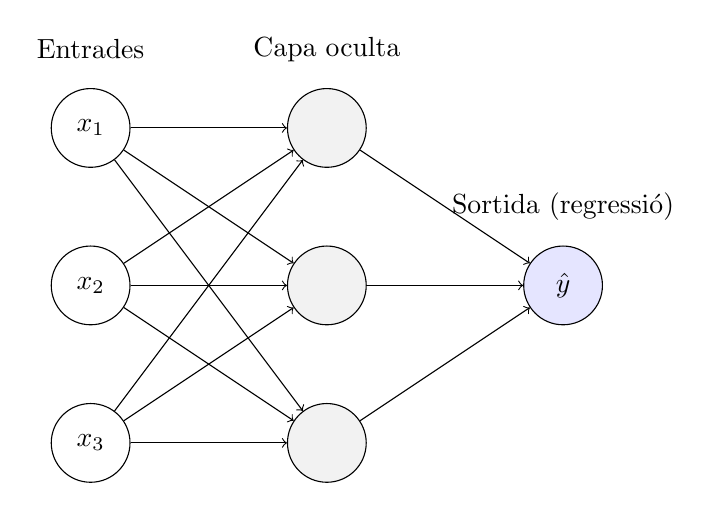
\begin{tikzpicture}[scale=1, transform shape]

% Input layer
\node[circle, draw, minimum size=1cm] (I1) at (0,2) {$x_1$};
\node[circle, draw, minimum size=1cm] (I2) at (0,0) {$x_2$};
\node[circle, draw, minimum size=1cm] (I3) at (0,-2) {$x_3$};

% Hidden layer
\node[circle, draw, fill=gray!10, minimum size=1cm] (H1) at (3,2) {};
\node[circle, draw, fill=gray!10, minimum size=1cm] (H2) at (3,0) {};
\node[circle, draw, fill=gray!10, minimum size=1cm] (H3) at (3,-2) {};

% Output layer
\node[circle, draw, fill=blue!10, minimum size=1cm] (O1) at (6,0) {$\hat{y}$};

% Connections input -> hidden
\foreach \i in {1,2,3}
  \foreach \h in {1,2,3}
    \draw[->] (I\i) -- (H\h);

% Connections hidden -> output
\foreach \h in {1,2,3}
  \draw[->] (H\h) -- (O1);

% Labels
\node at (0,3) {Entrades};
\node at (3,3) {Capa oculta};
\node at (6,1) {Sortida (regressió)};

\end{tikzpicture}
\caption{Esquema d’una xarxa neuronal de regressió}
\end{figure}

\section{Xarxa Neuronal amb llenguatge de programació}\label{sec:10}
En aquest apartat explicarem pas a pas de com vaig crear el nostre xarxa neuronal de regressió amb un llenguatge de programació.

\subsection{De celcius a fahrenheit}

Abans de començar a treballar amb la xarxa neuronal definitiu, vaig voler fer una de més simple per tal de coneixer amb més profunditat de com funciona una xarxa neuronal de regressió; en aquest cas he escollit un transformador d'unitats de temperatura, de celcius (\textbf{Unitat de temperatura basada en el punt de fusió de l'aigua}) a fahrenheit (\textbf{Sistema d'unitat basada en el punt d'ebullició i solidificació de l'aigua}). Per crear aquesta xarxa vaig escollir el Python com a llenguatge de programació, i el motiu esta explicat en l'apartat \ref{sec:4.4}.\\


Per començar, importo el framework i la biblioteca de Python que són les bases de dades necessàries per a la creació de la xarxa neuronal: \texttt{TensorFlow} (\textbf{framework}) i \texttt{{numpy}} (\textbf{biblioteca}). Com podeu veure, he creat uns \textit{abrevacions} per a poder-los cridar més fàcilment quan els necessiti.

\begin{itemize}
 \item \textbf{TensorFlow: } TensorFlow és un tipus de framework en que ofereix eines per crear i entrenar models de Ml (Machine learning) i Dl (Deep learning), biblioteques per programar xarxes neuronals i altres algoritmes, Compatibilitat amb GPU i TPU per accelerar càlculs, TensorBoard per visualitzar i monitorar entrenaments, Models preentrenats i repositoris, APIs (Application Programming Interface) en diversos llenguatges.
 \item \textbf{numpy: } numpy és una biblioteca científica per treballar amb vectors i matrius.
\end{itemize}
\begin{figure}[H]
    \centering
    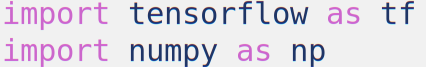
\includegraphics[width=0.5\textwidth]{./figures/1.png}
    \caption{Framework i biblioteca del Python}
\end{figure}


Agafo les paraules \textbf{celsius} i \textbf{fahrenheit} i les defineixo com a variables amb un signe \texttt{=}. Després poso \texttt{np} per indicar la biblioteca, seguit de \texttt{.array()} per especificar que és una llista. Dins dels parèntesis hi poso \texttt{[ ]} i a dins, els diferents valors de temperatura. Finalment, afegeixo el paràmetre \texttt{dtype=float} per indicar que es tracta de dades numèriques decimals.

Repeteixo el mateix procés amb \textbf{fahrenheit}, però en aquest cas les dades no poden ser arbitràries, sinó que han de ser les temperatures corresponents a les de \textbf{celsius} convertides a Fahrenheit. D’aquesta manera, la xarxa neuronal pot entendre la relació entre les dues sèries de dades.


\begin{figure}[H]
    \centering
    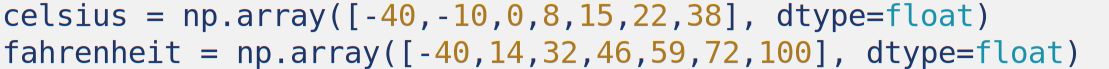
\includegraphics[width=0.5\textwidth]{./figures/2.png}
    \caption{Agrupació de dades amb numpy}
\end{figure}

Per començar, defineixo les capes de la xarxa neuronal. Utilitzant \texttt{tf.keras.layers.Dense} (\textbf{funció per a capes denses} (Keras és un tipus de API)), creo la primera capa oculta amb el paràmetre \texttt{units=3} per especificar que tingui \textbf{3 neurones}, i \texttt{input\_shape=[1]} per indicar que l'entrada és un sol valor. Li assigno el nom \texttt{oculte\_1}.\\ \\
Repeteixo el procés per a la segona capa oculta, \texttt{oculte\_2}, amb \texttt{units=3} neurones també, però sense especificar \texttt{input\_shape} ja que la xarxa ho dedueix automàticament de la capa anterior.\\ \\
Finalment, defineixo la capa de \texttt{sortida} amb \texttt{units=1} perquè retorni un sol valor (la predicció en Fahrenheit).\\ \\
Amb totes les capes creades, les integro en un model seqüencial amb \texttt{tf.keras.Sequential}, passant-les dins d'una llista \texttt{[ ]} en l'ordre correcte: \texttt{[oculte\_1, oculte\_2, sortida]}. Això crea l'estructura bàsica de la nostra xarxa neuronal.


\begin{figure}[H]
    \centering
    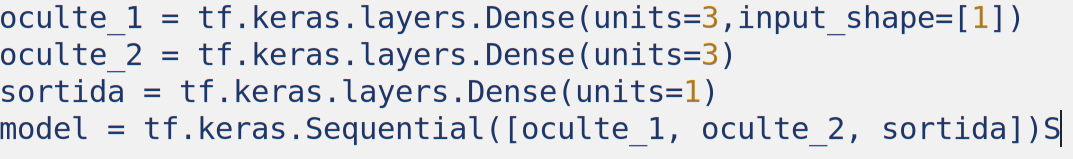
\includegraphics[width=0.5\textwidth]{./figures/3.png}
    \caption{Capes ocultes i la sortida d'una xarxa neuronal}
\end{figure}


Després de dissenyar l’estructura de la xarxa neuronal, cal ensenyar al model com aprendre i entrenar-se.
Per fer-ho utilitzem la variable \textbf{model}, a la qual ja havíem assignat les capes ocultes i la capa de sortida.
Tot seguit afegim la instrucció \textbf{.compile()}, que serveix per configurar el model abans de començar l’entrenament.

Dins de \texttt{.compile()} especifiquem el paràmetre \textbf{optimizer}, que indica la manera com el model ajustarà els pesos.
En aquest cas utilitzem \texttt{"adam"}, un optimitzador adaptatiu que redueix la velocitat d’aprenentatge quan detecta canvis bruscos en un pes,
l’augmenta quan el pes és estable i, alhora, recorda la direcció correcta per evitar oscil·lacions innecessàries.

A continuació, definim la funció de pèrdua amb el paràmetre \textbf{loss=\texttt{"mean\_squared\_error"}}.
La funció de pèrdua (\textit{loss}) mesura l’error del model i guia el procés d’aprenentatge.
En aquest cas, l’opció \texttt{mean squared error} (MSE, error quadràtic mitjà) és especialment útil en problemes de regressió,
ja que penalitza més fortament els errors grans i permet aconseguir prediccions més precises.


\begin{figure}[H]
    \centering
    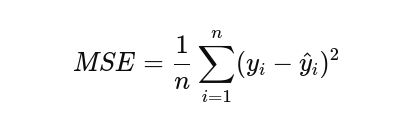
\includegraphics[width=0.5\textwidth]{./figures/5.png}
    \caption{Funció de pèrdua}
\end{figure}


\begin{figure}[H]
    \centering
    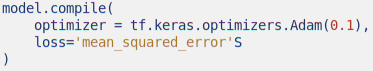
\includegraphics[width=0.5\textwidth]{./figures/4.png}
    \caption{Optimizació de la xarxa neuronal}
\end{figure}

Ara cal incloure la part crucial d'una xarxa neuronal: l'entrenament. Per fer-ho, utilitzem la variable \texttt{historial} per guardar l'evolució de l'entrenament i el model definit, \texttt{model}, aplicant-li el mètode \texttt{.fit()} que es el atribut que indica entrenament. Dins \texttt{.fit()} especifiquem, en ordre, les dades d'entrada (\texttt{celcius}), les dades de sortida (\texttt{fahrenheit}), el nombre de vegades que s'entrenarà la xarxa (\texttt{epochs=100}) i si volem mostrar el procés per pantalla (\texttt{verbose=1}, on 1 significa que sí i 0 que no).

A més, podem utilitzar \texttt{print()} per escriure comentaris o textos al terminal; en aquest cas hem posat \texttt{"Començem a entrenar..."} abans de començar i \texttt{"Model entrenat!"} un cop finalitzat l'entrenament.

\begin{figure}[H]
    \centering
    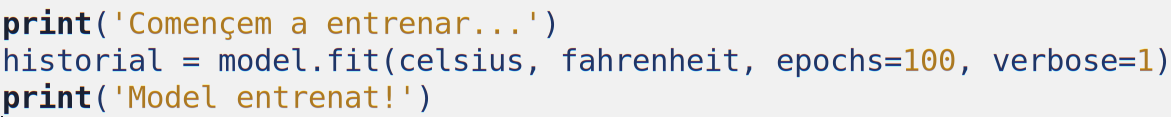
\includegraphics[width=0.5\textwidth]{./figures/6.png}
    \caption{L'entrenament de la xarxa neuronal}
\end{figure}

Després d’haver entrenat la xarxa neuronal i emmagatzemat l’evolució de la pèrdua a la variable \texttt{historial}, podem visualitzar com ha canviat la pèrdua a cada època utilitzant \texttt{matplotlib.pyplot}, una biblioteca de Python per crear gràfiques.

Primer, importem la biblioteca amb \texttt{import matplotlib.pyplot as plt}. A continuació, etiquetem els eixos de la gràfica amb \texttt{plt.xlabel("\# Època")} i \texttt{plt.ylabel("Magnitud de pèrdua")} per indicar què representa cada eix.

Per dibuixar la corba de la pèrdua utilitzem \texttt{plt.plot(historial.history[``loss''])}, que accedeix a la llista de valors de pèrdua que Keras ha guardat per cada època durant l’entrenament. Finalment, amb \texttt{plt.show()} mostrem la gràfica en una finestra del terminal o del notebook.

D’aquesta manera podem observar visualment si el model aprèn correctament, com disminueix la pèrdua al llarg de les èpoques i si hi ha comportaments irregulars que requeririen ajustar els paràmetres d’entrenament.

\begin{figure}[H]
    \centering
    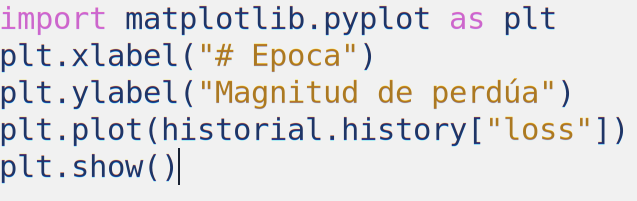
\includegraphics[width=0.5\textwidth]{./figures/7.png}
    \caption{La corba de pèrdua}
\end{figure}

Després d’haver entrenat la xarxa neuronal, podem fer prediccions amb nous valors d’entrada. Primer, utilitzem \texttt{print("Fem una predicció!")} per mostrar un missatge al terminal indicant que comença la predicció.

A continuació, fem servir \texttt{model.predict()} per calcular la predicció de la xarxa neuronal. En aquest cas, introduïm un valor de 100 graus Celsius amb \texttt{np.array([[100.0]], dtype=float)}, assegurant-nos que sigui un valor numèric decimal. El resultat s’emmagatzema a la variable \texttt{resultat}.

Finalment, utilitzem \texttt{print("El resultat es " + str(resultat) + " fahrenheit")} per mostrar la predicció obtinguda en Fahrenheit(el str es perque el variable resultat no sigui numeric sino un text). D’aquesta manera podem veure com el model converteix qualsevol temperatura de Celsius a Fahrenheit després de l’entrenament.


\begin{figure}[H]
    \centering
    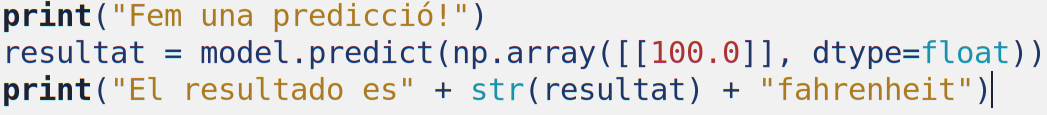
\includegraphics[width=0.5\textwidth]{./figures/8.png}
    \caption{Resultat de la predicció}
\end{figure}

Per a inspeccionar els pesos interns de la xarxa neuronal, podem utilitzar el mètode \texttt{.get\_weights()} en cada capa. Si el posem en els variables que haviem assignat les capes, per exemple, \texttt{oculte\_1.get\_weights()}, \texttt{oculte\_2.get\_weights()} i \texttt{sortida.get\_weights()} permeten veure els valors dels pesos i els biaixos que el model ha après durant l’entrenament, mostrant-los amb \texttt{print()}.


\begin{figure}[H]
    \centering
    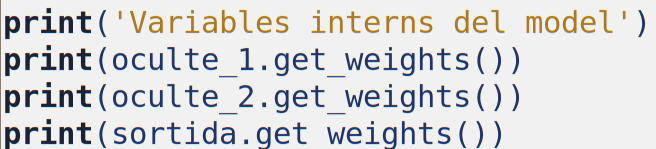
\includegraphics[width=0.5\textwidth]{./figures/9.png}
    \caption{Resultat de la predicció}
\end{figure}

Font: (\href{https://www.youtube.com/watch?v=iX_on3VxZzkhttps://www.youtube.com/watch?v=iX_on3VxZzk}{Xarxa neuronal amb Python})

\subsection{Predicció de les notes finals de matematiques }
Una vegada treballat amb la xarxa neuronal de celcius a fahrenheit, ja em trobo capacitat per fer la xarxa neuronal que ens haviem proposat, explicat en l'apartat \ref{sec:intr}




\section{Xarxa Neuronal amb fulls de calculs}\label{sec:11}
En aquest apartat continuarem amb la xarxa neuranal de regressió però aquesta vegada utilizarem un full de calculs per fer-ho.
L'estructura que utilitzarem per aquesta pràctica serà la del perceptró.

\begin{figure}[H]
    \centering
    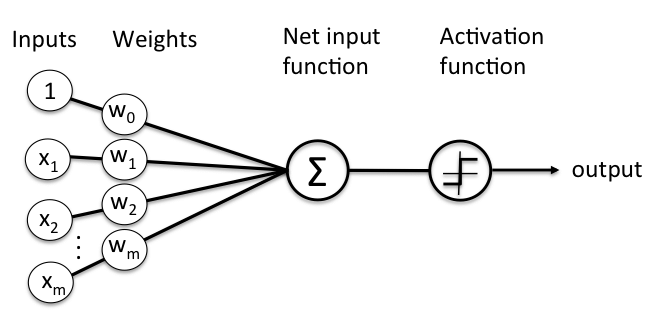
\includegraphics[width=0.5\textwidth]{./figures/perceptro.png}
    \caption{Estructura del perceptró}aaa
\end{figure}

Un cop sabem quina estructura utilitzarem, començarem la pràctica ordenant les dades de cada alumne del formulari en el full de càlculs

\begin{figure}[H]
    \centering
    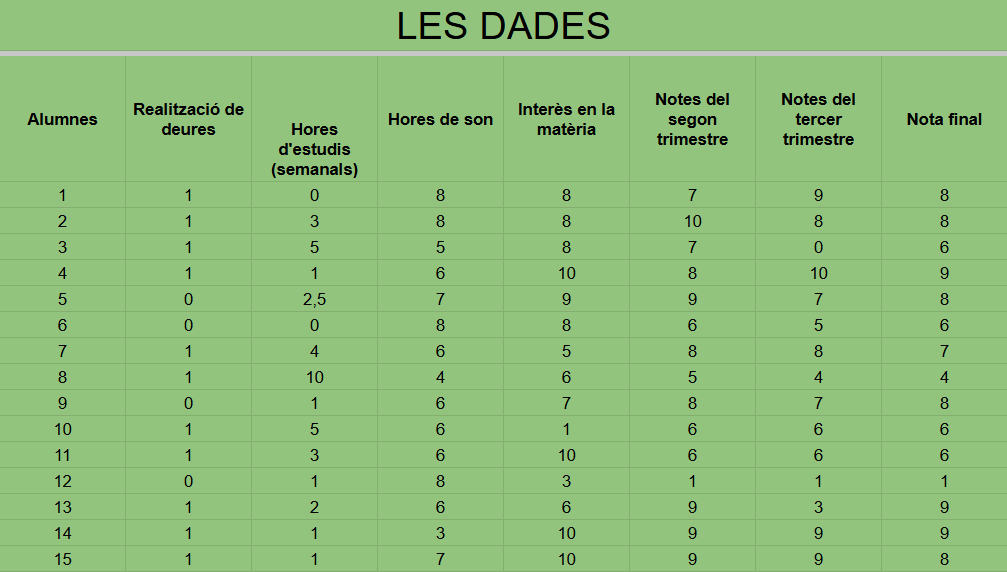
\includegraphics[width=0.5\textwidth]{./figures/Dades.png}
    \caption{Dades dels alumnes en el full de càlcul}
\end{figure}

Una vegada he ordenat tota la informació, he decidit representar els valors d'entrada d'una forma més senzilla d'entendre i curta, anomenantlos $xi$
\begin{itemize}
 \item \textbf Realització de deures: $x1$
 \item \textbf Hores d'estudis: $x2$
 \item \textbf Hores de son: $x3$
 \item \textbf Interès en la matèria: $x4$
 \item \textbf Notes del segon trimestre: $x5$
 \item \textbf Notes del tercer trimestre: $x6$
 \item \textbf Nota final: $y$
\end{itemize}

Aquestra representació queda així:

\begin{figure}[H]
    \centering
    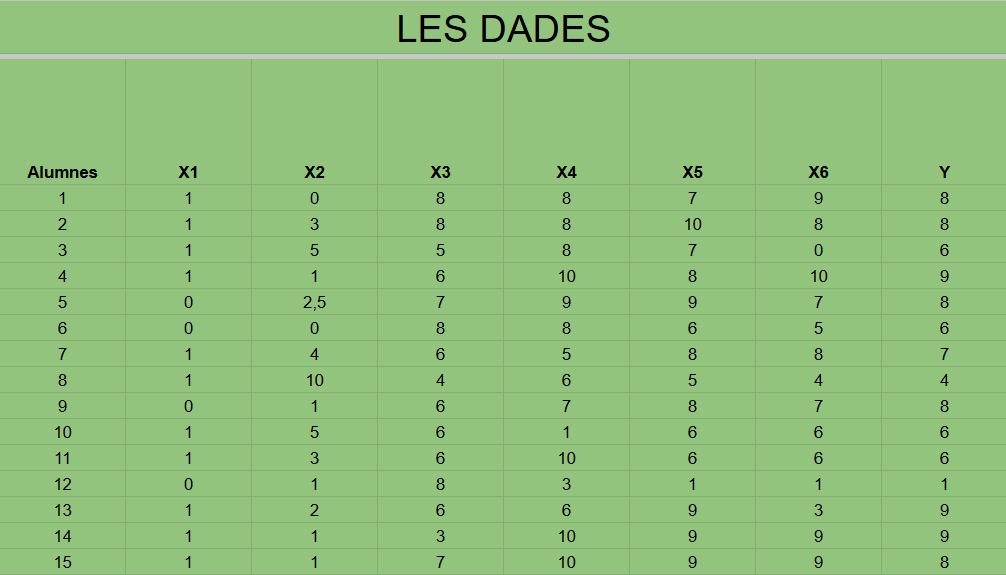
\includegraphics[width=0.5\textwidth]{./figures/Dades_resumides.png}
    \caption{Taula resumida}
\end{figure}

L'entrada de ``Realització de deures'' és una data binaria que nomès pot prendre valors 0 o 1.
\subsection{Normalització de dades}
Abans de continuar, és necessari explicar que és la normalització de dades.
La normalització de dades és una tècnica de procesament que consisteix en transformar dades de diferents escales a una escala comú, com per exemple del 0 al 1, aixó facilita la comparació i l'anàlisi de la xarxa neuronal i millora el seu rendiment. En el nostre cas, tenim dades binaries i dades ordinaries qe poden prendre qualsevol valor, aquest desequilibri afecta els càlculs posteriors si no es solucionen d'alguna manera.

Per aquesta raó, convertirem totes les dades en valors d'entre 0 i 1. Aquest procès implica calcular la miitjana de les dades i la desviació estàndar de cada variable. Per això utilitzant la fòrmula seguent:\\
$z = \frac{x - \mu}{\sigma}$\\

On:\\
$z$ És el valor normalitzat\\
$x$ És el valor original\\
$\mu$ És la mitjançan\\
$\sigma$ És la desviació estàndar\\

Aquests càlculs són fàcils d'obtenir amb les funcions que ens proporciona el full de càlcul.

\begin{figure}[H]
    \centering
    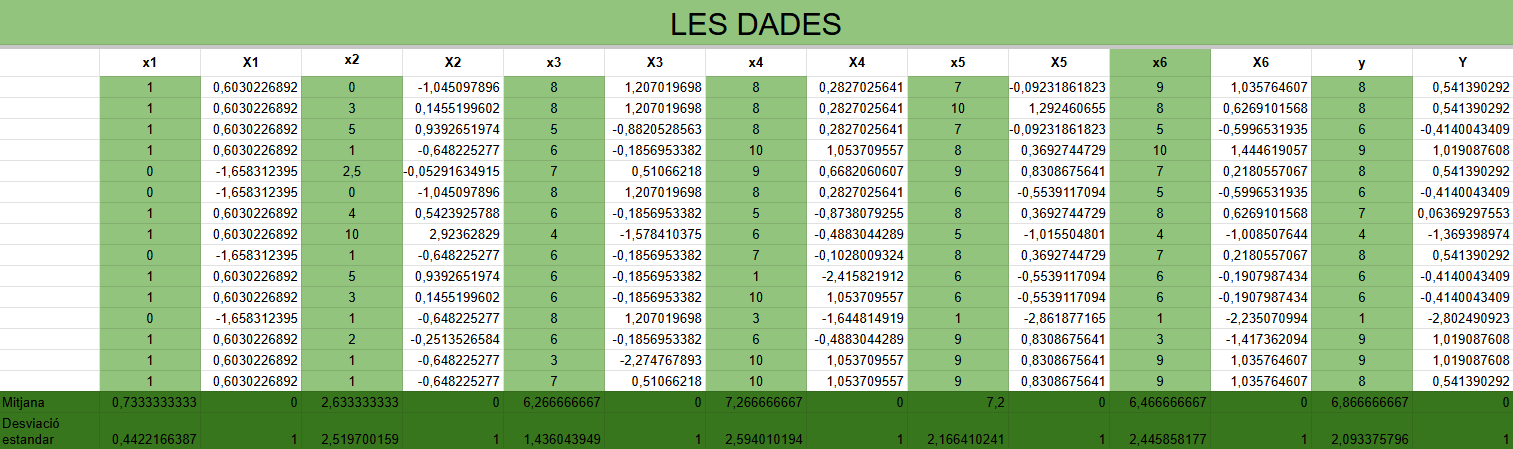
\includegraphics[width=0.5\textwidth]{./figures/Dades_normalitzades.png}
    \caption{Taula resumida}
\end{figure}

\subsection{Els pesos}
En una xarxa neuronal, cada valor d'entrada té el seu respectiu pes que determina la importància que té en la predicció final. AL començament de l'entrenament, assignarem a tots els pesos el mateix valor, ja que aquests es corregiran lentament durant el procès de l'entrenament.

\begin{figure}[H]
    \centering
    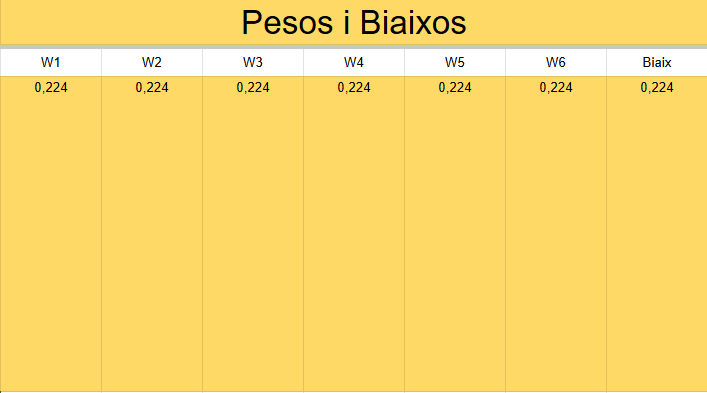
\includegraphics[width=0.5\textwidth]{./figures/Pesos.png}
    \caption{Taula dels pesos}
\end{figure}

Com es pot veure a la figura 6.9, he afegit 6 columnes pels pesos, respecte als 6 valors d'entrada, tambè he afegit una columna pel biaix, que serà la constant per millorar l'aust de les prediccions.

\subsection{Funció de pèrdua}
Ara que ja tenim les dades normalitzades i hem assignat els sues respectius pesos inicials, podrem aplicar la fòrmula de les xarxes neurnals artificials per calcular la predicció de les notes dels alumnes.
Recordem que la fòrmula de les xarxes neuronals artificials és:\\
\[
\sum w_i x_i + \text{biaix}
\]\\
Després d'aplicar aquesta fòrmula, obtindrem les prediccions de la nota final, tal com es mostra en la figura seguent.

\begin{figure}[H]
    \centering
    \includegraphics[width=0.5\textwidth]{./figures/Predicció.png}
    \caption{Prediccions del model}
\end{figure}

Cal recordar que aquest valors de la predicció són provisionals, ja que el valor dels pesos encara són imprecises.

El següent pas és entrenar el model per ajustar els pesos i fer més precís els valors de la predicció de la xarxa neuronal, per aconseguir-ho, utilitzarem un mètode d'optimització per ajustar els valors dels pesos, en aquest cas utilitzarem l'algoritme gradient descendent per minimitzar la funció d'error.

Per poder apicar aquest algoritme haurem d'afegir més columnes al nostre full de càlcul. Si restem els valors de la predicció ($Y$), amb els valors reals ($y$) obtindrem la diferència de la nota, es a dir, l'error del model.

\begin{figure}[H]
    \centering
    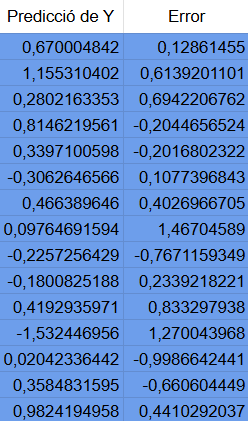
\includegraphics[width=0.5\textwidth]{./figures/Errors.png}
    \caption{Taula d'errors}
\end{figure}

Com podem veure en la figura 6.11, hem afegit 2 taules més, la taula d'error, on s'emmagatzema els errors del model, i la taula d'errors en positiu, aquesta última taula recull les dades de la taula d'error i agafa el valor absolut de les dades, fent que tots els valors es tornin positius, d'aquesta manera facilita els càlculs a l'hora de cambiar els paràmetres i s'aprecia la diferència de la predicció i el valor original.

Després d'aquest pas calcularem la mitjana de la taula dels errors en positius. El valor que dongui la mitjana ens ajudarà a saber si la xarxa està millorant la seva precisió, si aquest valor és petit, vol dir que l'error també és petit, fent el model més precís, en cada iteració hem d'aconseguir minimitzar aquest valor perquè el model sigui ho més precís possible.

\subsection{Canvis dels paràmetres}
Ara que ja sabem les funcions d'error de la primera predicció, ens toca entrenar el model per ajustar els pesos per disminuir els errors. Per dur aixó hem de tindre en compte ho següent: Com hem vist abans, l'error del model és la diferència que hi ha entre la predicció ($Y$) i el valor real ($y$), aixó vol dir que quan més gran sigui aquesta diferència, els pesos estaran més lluny del seu valor adequat, hem de trobar una forma per reduïr la diferència d'aquests valors.
Per altra banda, els valors d'entrada ($X$) es multipliquen pels seus respectius pesos ($W$), això vol dir que si el valor d'entrada ($X$) és petit, el seu pes ($W$) també serà petit, ja que aquests es multipliquen, com ho diu la fòrmula.
Per tant hem de tindre en compte dues coses: La diferència entre la predicció ($Y$) y el valor real ($y$) i el valor d'entrada ($X$) respecte a cada pes ($W$). Així que la fòrmula que utilitzarem per calcular els canvis de cada paràmetre serà:

\section{Comparació entre una xarxa neurnal creada per un llenguatge de programació netre una de fulls de calculs}

\section{Xarxa Neuronal amb un cas real}\label{sec:12}
